\section{DDlog Implementation}\label{sec-system}

\subsection{Compiling DDlog to Differential Dataflow}

\paragraph{Differential Dataflow}
The core execution engine of DDlog is Differential Dataflow (DD).
Differential Dataflow~\cite{differential-dataflow-paper} is a
streaming big-data processing system which provides incremental
(differential) computation.  DD is an \emph{incremental}
map-reduce-like system, but supporting a wide set of relational
operators, including recursion (fixed-point) and joins.  Section 4.3
in~\cite{differential-dataflow-paper} describes the core relational
operators that are used by our compiler to implement DDlog operators.
DD is described in several
publications~\cite{timely-dataflow,differential-dataflow-paper} and
online documents~\cite{dd-mdbook,dd-reference}.  DD can be executed
using multiple cores or even multiple shared-nothing machines, but we
currently only support a single machine.

\paragraph{Compilation}
Figure~\ref{fig:compiler-flow} shows how DDlog programs are compiled.
The DDlog compiler is written in Haskell.  The compiler performs
parsing, type inference, validation, and several optimization steps;
it generates Rust code (as text files); the Rust code is compiled and
linked with the open-source Rust version of the DD
library~\cite{differential-dataflow}.

\begin{figure}
\begin{center}
    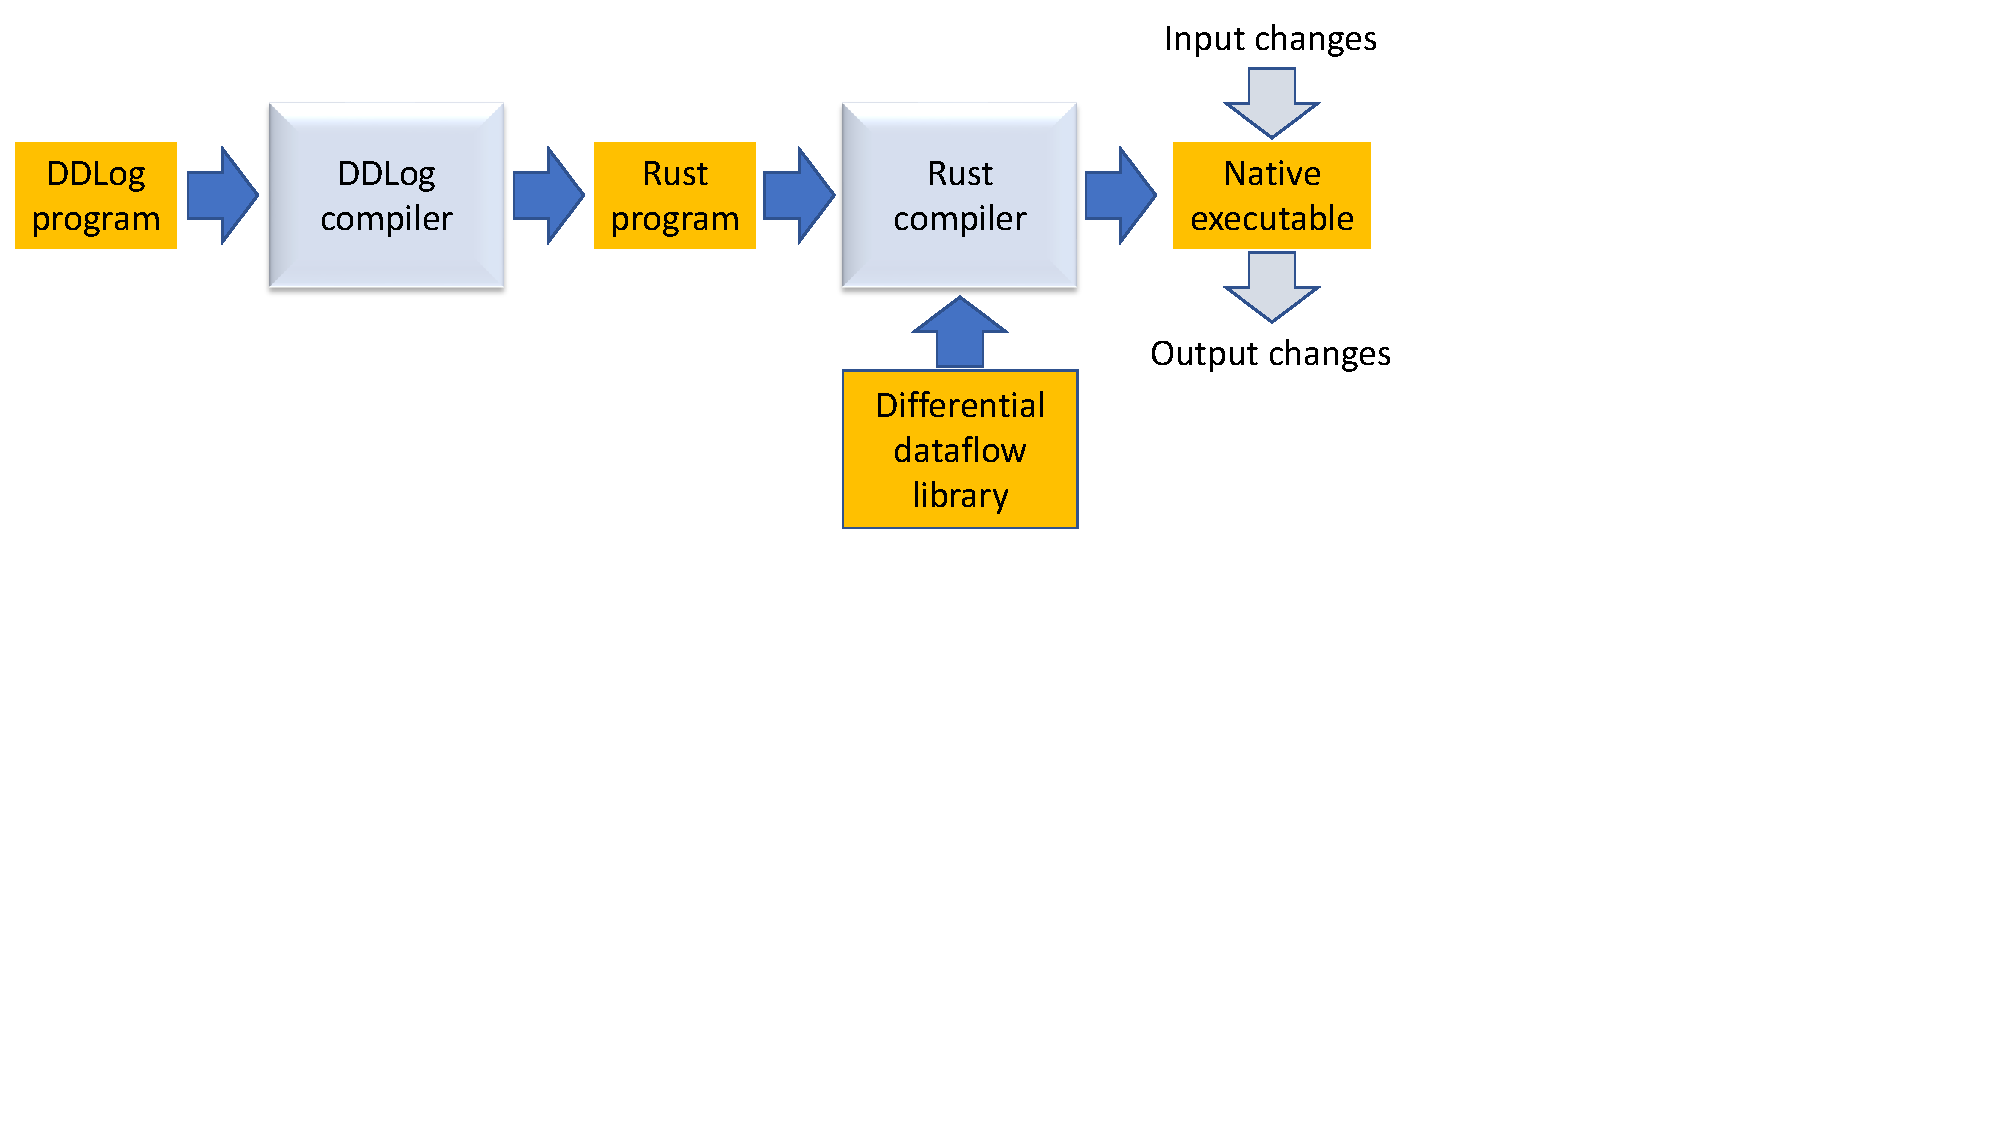
\includegraphics[width=.7\columnwidth,clip=true,trim=0in 4in 4in
      0in]{compiler-flow.pdf}
\end{center}
    \caption{DDlog compilation flow.\label{fig:compiler-flow}}
\end{figure}

The output of the DDlog compiler, and the input to the DD library is a
dataflow graph, which may contain cycles (introduced by
recursion).  The nodes of the graph represent relations are dataflow
relational operators; edges connect operators to their input and output
relations.  DD natively implements
the following operators: join, antijoin, union, aggregation,
filter, and flatmap.  Each operator has a highly optimized
implementation, incorporating temporal indexes that track
updates to each relation over time and allow efficient incremental evaluation.
The DD library is responsible for executing the emitted
dataflow graph across many cores.  The
DD runtime can be configured with one or more worker threads.

\subsection{Interacting with DDlog programs}

\paragraph{Transactional API}
The interaction with a running DDlog program is done through a
transactional API.  At any time only one transaction can be
outstanding.  After \texttt{start}ing a transaction the user can
insert and delete any number of tuples from input relations.  When
attempting to \texttt{commit} a transaction all updates are applied
atomically and changes to all output relations are produced.  Users
can register an upcall to be notified of these changes.
%These
%notifications will happen on different threads, while the thread
%executing the \texttt{commit} is blocked.
Figure~\ref{fig:javaapi}
shows an example Java program that interacts with a DDlog program.

\paragraph{The command-line interface}
For every DDlog program the compiler generates a static or dynamic library
(depending on user-provided compiler flags), that exports the transactional API
to the DDlog program, which can be
invoked from Rust or other languages, and a
command-line interface program (CLI) that allows users to interact
with the DDlog program directly via a command line or a command file.
The CLI allows users to start
transactions, insert or delete tuples in input relations, commit
transactions, dump the contents of relations, and get statistics
about resource consumption.  The CLI is used for regression testing
and debugging.

\paragraph{C and Java interfaces}
The DDlog API is natively
implemented in Rust, with bindings available for other languages,
currently C and Java.
We illustrate the Java API to a simple DDlog program with a
skeleton example in Figure~\ref{fig:javaapi}.

\begin{figure}
  \footnotesize
  \begin{lstlisting}[language=ddlog]
// DDlog program
input relation Parent(parent: string, child: string)
output relation Ancestor(ancestor: string, descendant: string)
Ancestor(ancestor, descendant) :- Parent(ancestor, descendant).
Ancestor(ancestor, descendant) :- Ancestor(ancestor0, ancestor1),
                                  Parent(ancestor1, descendant).
  \end{lstlisting}

  \begin{lstlisting}[language=Java]
// Java program interfacing with DDlog program
static class Parent {
  String parent;
  String child; }
static class Ancestor {
  String ancestor;
  String descendant; }

/* Instantiate the DDlog program; add a record to the
 * Parent relation. */
static void main() {
  DDlogAPI api = new DDlogAPI(2 /* threads */,
               r -> onCommit(r) /* callback */);
  int parentRelation = api.getTable("Parent");
  Parent p = new Parent();
  p.parent = "Mike"; p.child  = "John";
  /* Create DDlog insert command. */
  DDlogCommand command = new DDlogCommand(
     DDlogCommand.Kind.Insert, parentRelation, p);
  int exitcode = api.start();  // start transaction
  DDlogCommand[] commands = new DDlogCommands[1];
  commands[0] = command;
  exitcode = api.applyUpdates(commands);
  /* commit transaction; causes the callback to be
   * invoked for each new or deleted output record.
   * commit blocks until all upcalls have been invoked. */
  exitcode = api.commit();
  api.stop();
}

/* Callback invoked on commit once for each insertion or
 * deletion in an output relation. */
static void onCommit(DDlogCommand command) {
  int outputRelation = command.tableId;
  Ancestor value = command.getObject<Ancestor>();
  if (command.kind == DDlogCommand.Kind.Insert)
    // ancestor inserted
  else
    // ancestor deleted
}
\end{lstlisting}
\caption{Example program showing the Java API to pass and receive data
  from a DDlog program.\label{fig:javaapi}}
\end{figure}
